\documentclass[a4paper,10pt]{report}
\usepackage[utf8]{inputenc}
\usepackage[top=3cm, bottom=2.5cm, left=2cm, right=2cm]{geometry}
\usepackage{colortbl}
\usepackage{color}
\usepackage[pdftex]{graphicx}
% Title Page
\title{WebAgenda User Guide}
\author{Daniel Kettle, Noorin Hasan, Mark Hazlett, Daniel Wehr}

\definecolor{note}{rgb}{0,0.35,0} 

\begin{document}
\maketitle
\tableofcontents
\setcounter{chapter}{-1}
\chapter{Preamble}

\par \noindent \hspace*{1cm} WebAgenda is a Web-Hosted scheduling system that is meant to provide scheduling, employee tracking, and report generation to any business. It is built to fit small to medium businesses, although is not limited by business size.  This User Guide will go through operation and guidelines while using and implementing the system for a business. This manual is aimed at the business owner who has fair experience with computers. It is recommended that they have a server in place or hand this guide off to someone who can set one up for them. Installation is fairly straightfoward and this guide will go over concepts in some depth in an outlined box. Any notes, warnings, or serious issues you may encounter or should consider will be printed in a green, orange, or red font respectively. 

\begin{quote}
WebAgenda version 0.99 Beta, Copyright (C) 2009-2010 Daniel Kettle, Daniel Wehr, Mark Hazlet, Noorin Hasan.
WebAgenda comes with ABSOLUTELY NO WARRANTY. \\
This is free software, and you are welcome to redistribute it under certain conditions. See License section in the Appendix for more information.
\end{quote}



\chapter{Installation}

\par \noindent \hspace*{1cm} The \textit{complete} installation requires third-party programs as well as the WebAgenda application. These extra programs are included with the installation discs, but may not be licensed under the same terms nor distributed under the same rules. As such, licenses are displayed in the appendix of this manual and the installer launches each individual program installer independant of itself. Included third-party applications are Windows 32-bit only as the test environment and quite possibly most of the business systems we expect this program to be installed on will be. Apple or *nix server administrators should be able to install the respective \textbf{MySQL},\textbf{Glassfish} and \textbf{Java EE} programs easily. 
\bigskip
\par \noindent \hspace*{1cm} The WebAgenda Official Windows Installer is 32-bit only currently and includes Java EE 6 plus Glassfish v3, MySQL 5.1.x RDBMS database, and the actual WebAgenda files. In order to install WebAgenda, you must accept the license agreement of the GNU Public License found in the Appendix section of this guide (text in full).

\section{Minimum Requirements}
\subsection*{Windows XP and Greater}
% TODO Re-order reqirements into a standard order
\begin{itemize}
 \item 500 MB free space 
 \item 1024 MB RAM
 \item 2.0 GHz Dual Core processor
 \item Network Connectivity, 100 Mbps connection minimum
 \item 32 MB Video RAM
 \item UTF-8 Language Support
\end{itemize}

\subsection*{Mac OS-X 10.5 and Greater}

% See above TODO

\begin{itemize}
 \item 640 MB free space
 \item 1024 MB RAM
 \item 2.0 GHz Dual Core processor
 \item Network Connectivity, 100 Mbps connection minimum
 \item 32 MB Video RAM
 \item UTF-8 Language Support
\end{itemize}

\subsection*{GNU/Linux (Kernel 2.6+), BSD, Unix}

\begin{itemize}
 \item 500 MB free space
 \item 512 - 1024 MB RAM *
 \item 1.5 - 2.0 GHz Dual Core processor *
 \item Network Connectivity, 100 Mbps
 \item 16 - 32 MB Vido RAM *
 \item UTF-8 Language Support
\end{itemize}

\begin{small} * Lower requirements if system is command-line only \end{small}
\paragraph{}

% This is a Note
\begin{color}{note}
\begin{center}
\begin{tabular}{| l |}
\hline
  \begin{footnotesize}
  Mac OS-X should have MySQL installed by default and Apple customizes Java for their machines. 
  \end{footnotesize} \\
  \begin{footnotesize}
  Most GNU/Linux servers should have a respective repository or source code to build from.
  \end{footnotesize} \\
  \begin{footnotesize}
  Unix Systems may not have repositories, but should be able to make use of source code.
  \end{footnotesize} \\
  \begin{footnotesize}
   Solaris and embedded systems have not been tested with WebAgenda.
  \end{footnotesize} \\
\hline
\end{tabular}
\end{center}
% End Note
\end{color}
\par \noindent \hspace*{1cm} 


\chapter{First Run}

\par \noindent \hspace*{1cm} Once the installer has been run and all dependencies are installed, WebAgenda should be accessible. The site can be reached if installed on a local machine at:
\begin{center}
 \texttt{http://localhost:8080/WebAgenda/} (might want to change this for final)
\end{center}


\section{Business Components Overview}
\par \noindent \hspace*{1cm} WebAgenda will require some post-installation setup before it can be used 
\subsection{Physical Locations}

\par \noindent \hspace*{1cm} Some businesses may be spread over multiple physical locations and have employees not limited to one. The Location that is referred to in WebAgenda is a piece of information that allows a Job to be tied to a physical location, so similiar jobs that are required simultaneouly in different locations can be scheduled.
\bigskip
\par \noindent \hspace*{1cm} Locations consist of a name that identifies the location and a description. It is recommended that the address of the physical location be included in the description so that the name can be in an easily accessible short form format.
\begin{verbatim}
      Name: SW11
      Description: Floor 11 of Hotel Sleepwell
\end{verbatim}

\begin{verbatim}
      Name: Main Lobby 5392 FAC 
      Description: 5392 Fake City Dr., Financial Accounting Centre, Main Lobby
\end{verbatim}

\par \noindent \hspace*{1cm} Of course, a Location does not have to have a description. This can be left blank as long as the name is unique. Searches that are performed based on tags such as \texttt{Lobby, Accounting,} and \texttt{5293} should all return the second example`s Location.

\subsection{Job Roles}

\par \noindent \hspace*{1cm} A Job Role is called a Position by WebAgenda and is basically the job description that is tied to a Location. Multiple Positions can be associated with a Location. Similarly to the Location, a Position has a unique Name and an optional Description.

\begin{verbatim}
      Name: Cleaner
      Description: Cleaner for Hotel Sleepwell specific to one floor
\end{verbatim}

\begin{verbatim}
      Name: Financial Accountant
      Description: Someone who does accounting
\end{verbatim}

\par \noindent \hspace*{1cm} The above examples do not cover all possible scenarios how a Position can be used.

\subsection{Job Skills}

\par \noindent \hspace*{1cm} A Skill is part of a Position; It's an optional requirement when limitations are placed on the Position. Skills mainly affect how the scheduling is performed, the automatic schedule generation in particular. By assigning a Skill to a Position, only Employees who have been assigned that Skill by someone in authority such as their supervisor, manager, or administrator can work that job. One of the more obvious uses for a Skill is when some jobs require handling and / or serving of liquor that requires an Employee to be of proper age. 

\begin{verbatim}
      Name: Bartender
      Description: Server liquor to customers in restaurant
\end{verbatim}

\par \noindent \hspace*{1cm} A Skill does not have to have a description in it, nor does a Position require any skills.

\subsection{Employees}

\par \noindent \hspace*{1cm} Employees contain mostly personal information when they are created along with security attributes, preferred work values, and their status (active, not active). An Employee has the ability to change some of the basic information about them, but much of it is handled by security or higher authorities in the system. Employees will start off with the lowest default security settings.
\bigskip
\par \noindent \hspace*{1cm} Most of the required information that is not handled by the system is stated below. While the date of birth of an employee is not required, these employees will not be factored into positions that require age limitations, such as the Bartender job (if applicable). It is important to note how permissions work in the system, which is detailed later on.

\begin{verbatim}
      First (Given) Name: Joe
      Last (Family) Name: Smith
      Date Of Birth (Optional) : yyyy-mm-dd
      Email : joe.smith@email.com
      Username : joe_the_man
      Password : ********
\end{verbatim}

\subsection{Shifts}

\par \noindent \hspace*{1cm} Shifts are a representation of time that an employee is placed in the schedule for. A Shift can be assigned to a Shift Template counterpart that holds a required position as well as time contstraints. The Template is used for auto-scheduling employees where they must be assigned to specific positions at specific times. As a schedule does not have to be auto-generated and can have employees placed in it manually, Templates are not specifically needed to fill a schedule shift. By manually creating a schedule, there are no dependencies on Positions or Templates, although there is no auto-generating schedule functionality as a result. 

\begin{verbatim}
      Time Start: 08:00:00
      Time End: 17:00:00
      Day of Shift: THURSDAY
\end{verbatim}

\par \noindent \hspace*{1cm} In addition to Shifts, a Shift Template contains a list of Shifts that is referenced by a Start Time and an End Time. A Template Shift is used in tandem with a Template Schedule to provide the framework for having one or more shifts applied to a Template Shift. 
\bigskip
\par \noindent \hspace*{1cm} When a Template Schedule is created, it becomes a blank schedule. By adding Template Shifts to different times on different days, they will mark the times that a shift is required in that time slot for an actual schedule when it is generating. A Template Shift can also associate itself with a Position, meaning that if someone needs to work in the bar every night from 10:00pm until midnight, a Shift Template can be set from 22:00 hours to 24:00 (or 00:00) hours with a required position of Bartender. Then, when generating a schedule (based off the schedule template), the system will look for Employees who can work at Bartending and set them at that point.
\bigskip
\par \noindent \hspace*{1cm} More than one Shift can be applied to a Shift Template on a Schedule Template object, but Shift Templates must be unique because there is no need to have multiples. Multiple Shifts can reference the same Template; There is a limit on the number of Employees who can be assigned to a Shift Template.
\bigskip
\par \noindent \hspace*{1cm} Shifts reference Shift Templates and Schedules reference Schedule Templates. A Shift Template will not be seen as a Shift.


\subsection{Scheduling}

\par \noindent \hspace*{1cm} A Schedule is a series of Shifts that make up the amount of work required within a specified period of time for the business. It is made up of the following values:

\begin{verbatim}
      Start Date: 2010-04-18
      End Date: 2010-04-24
\end{verbatim}


\par \noindent \hspace*{1cm} Scheduling is quite simply taking multiple Employees and assigning them to tasks known as Positions (that rely on a Location and possibly Skills) at a certain Time and Day. A schedule is a \textit{collection} of Shifts that relate to Employees involved in the result. The purpose of a Schedule Template is to produce a dynamically generated schedule based on the Employees currently in the system without requiring the labour of individually assigning an Employee to every Position required. Instead of having to create a Schedule every week or month or however the person in charge of creating them decides is best for their company, one template is created that can be generated whenever those Positions at the specified times are required. Create once and deploy multiple times, saving time and labour, therefore money. 
\bigskip 
\par \noindent \hspace*{1cm} Multiple Schedule Templates can be saved and used for later. A Christmas schedule, for example, may have vastly different Employee requirements then a summer schedule. In the end, all Templates are supposed to accomplish is to lighten the workload of creating schedules. 

\subsection{Permissions}

\begin{footnotesize}
\par \noindent \hspace*{1cm} The ability to change and assign permissions is absent in the current stable release; All modifications must be done through the database if they are required. All new Employees start with the lowest functioning set of permissions.
\end{footnotesize}
\bigskip
\par \noindent \hspace*{1cm} Permissions consist of two different parts: a 'level' value and a 'version' value. Most Employees can utilize the system just fine using the lowest permission defaults: a level of 0 and no version. However, once Employees become more specialized, especially in the areas of administration and schedule management, then versions may have useful application. In addition to level and version, there exists a list of permissions that can be toggled or set. All three elements combined are represented as a PermissionLevel, a complete permission entity assigned to an Employee.
\bigskip
\par \noindent \hspace*{1cm} The level attribute is an indication of how much authority the Employee has compared to other Employees in the system. Levels are hierarchical so even if the list of permissions are identical, a higher level will have priority and cannot be changed by lower level requests. 
\bigskip
\par \noindent \hspace*{1cm} The version represents a different set of Permissions that still retains the hierarchical structure of permission levels, but allows that level to focus on one aspect of the system. For example, if a company has three Employees in its employ, all of which are considered supervisors, one could be in control of scheduling while the other two are focused on hiring and reporting data from the system. It makes more sense to have the one supervisor in charge of scheduling to not have reporting functionality while the other two would lose schedule creation ability. This may negate performance losses from certain Employees attempting to utilize the database for non-critical activities. A version value is specified by an alphabetical character (a - z) or by a space if no version is desired. To emphasize, the version attribute is not taken into account when comparing levels.
\newpage
\par \noindent \hspace*{1cm} A PermissionLevel's level and version is not tied down to any particular combination of Permissions. Both levels and versions are based off \textit{explicit permissions} that determine what a user can or cannot do. These are assigned to employees by an administrator or someone with similar authoirty for the purpose of performing the related ability.
\par \noindent \hspace*{1cm} The following is a list of Permissions that limit how an Employee can use the system if it`s not enabled.

\begin{itemize}
 \item Can edit current or future schedules saved in the database.
 \item Can read the schedules. In the event of contract workers, they may not have a schedule.
 \item Can read past schedules. 
 \item Can manage employees. Able to change personal data, view permissions, disable login.
 \item Can view resources. Access to view employee data who have permission levels lower than user.
 \item Can change permission attributes. Only applicable to employees with levels lower than user.
 \item Can read logs. If implemented, view server logs on access violations, actions, etc.
 \item Can read reports generated by users as well as generate their own.
 \item Can request days off. (not implemented)
 \item Number of days off. (not implemented)
 \item Can request vacation days. (not implemented)
 \item Number of vacation days. (not implemented)
 \item Can take emergency days off. For adverse situations that cannot be planned.
 \item Can view inactive employees. 
 \item Can send notifications. Employees can send messages that show up on the main page after login.
 \item Trusted level. Temporarily increase a Permission`s level attribute to another user's level. \newline
 		(not implemented: Logging of actions while Employee has trusted status)
\end{itemize}



\section{Integrating Business Components}

\par \noindent \hspace*{1cm} In order to use WebAgenda, the following items must be set up: Employees, Permissions, Locations, Shifts and Schedules. By their very name, these business objects are self-explanatory. In this section, an example company will determine what of each object will be used in starting up their WebAgenda scheduling system.
\bigskip
\par \noindent \hspace*{1cm} There is a hotel startup that wants to be able to have a centralized scheduling system and they have chosen WebAgenda to perform that duty. They installed the software on their company's central server that can be accessed via the Internet and want their Employees to start using the system. This is their first time using the system.
\bigskip
\par \noindent \hspace*{1cm} The hotel is a small operation. There are 4 floors and a lobby as well as some administration offices. There are 30 staff that are employed in total not including the owner, 10 of which will be working at the hotel throughout a 12 hour period. 10 Employees won't be working at any one time unless the others are sick or on leave. As it is a small operation, the owner is lending the admin account of the system to the next highest authority figure in the business to perform scheduling and reporting. He expects the reports to be emailed to him every month. 

\subsection{Adding Employees}

\par \noindent \hspace*{1cm} The first task to getting the system up and running is to add all the employees into the system. The only personal information that is needed to get started is the first and last name, a username and a password. An e-mail is recommended as it can be used to send new passwords to as well as provide updates to schedules as they are made available. An Employee ID is a number value that can vary; 1-999 can be management, 1000-9999 can be regular workers for example.
\bigskip
\par \noindent \hspace*{1cm} There should be a Users link on the left sidebar in WebAgenda. That link leads to the page where new Employees can be created. Once the accounts have been set up, if e-mails were provided then the passwords to the accounts can be sent back through those addresses to the Employees. Verify the Employees have been created afterwards by searching for all employees.
\bigskip
\par \noindent \hspace*{1cm} By default, the Employees being created will have access to read the schedules and change trivial information about themselves. They will be prevented from accessing administrative abilities. The WebAgenda site should be available through any cellphone with a browser and javascript.

\subsection{Adding Positions}

\par \noindent \hspace*{1cm} Once the resources have been created, the next thing to do is create tasks for them. Tasks are in the form of Positions, places that must be worked. The hotel requires one Employee for every two floors to clean, 2 Employees at the front desk, and one manager in the offices. Each day consists of two 6-hour shifts for a total of 10 Employees. Positions that could gleaned from this example are Cleaners, Receptionists, Administration. Once these have been created, an Employee can be assigned to that Position.

\subsection{Adding Locations}

\par \noindent \hspace*{1cm} Locations, while optional for Positions, are recommended. There will always be two cleaners so it would be easier to recognize when one Employee has a Cleaning job on Floors 1-2 and Floors 3-4, rather than have two Employees who aren't sure of where they work when they arrive at the hotel.

\subsection{Adding Skills}

\par \noindent \hspace*{1cm} In the event that the schedule creator wants to restrict the job to one type of Employee, they can force a Position to require a Skill. A Skill is an attribute assigned to an Employee so that a Position can only be taken by one with that Skill. This tends to work more towards age-restricted jobs and auto-schedule generation.

\subsection{Final Mention}

\par \noindent \hspace*{1cm} The basics of setting up WebAgenda are mentioned above, but there are more features implemented although some aren't as full-featured yet. It's worth mentioning that there are reporting and schedule export features in this software. It's built on the GPL v2 license (included in this document, Appendix A) that allows developers to continue development without legal intimidation and unfair restrictions. Notifications are sent to Employees when new schedules are created or current ones modified (among other reasons), which are basically pop-ups on the main page after login that display important information. Among report generation, there is a way for administration and management to check the current activity of the Employees, so if problems arise with miscommunication or ill attendance, it can be determined if the system, or human error, is at fault.
\bigskip
\par \noindent \hspace*{1cm} More business components have been planned and it will be seen if they are integrated into the project. Functionality such as exporting to Open Document Format spread sheets and documents, pdf's, iCal, and some calendar formats would be a high priority as well as creating Roles for Jobs; they would be similar to Skills except use logical operations such as date of birth to determine age, rather than having a Skill that is monitored by management to ensure that no one lower than the legal age works at a limited Position.

\chapter{System Usage}

\chapter{Maintenance}

\section{Delete Instead of Disable Employees}

\par \noindent \hspace*{1cm} Employee data is never truly deleted from the WebAgenda system. Depending on the geographic location and government, records of employement may need to be stored for long periods of time. Tax records for instance, must be kept for 7 years in Canada. Therefore, there is no way to delete actual data from WebAgenda itself. In order to delete the data permanently, one must do so by logging into the database and deleting inactive employees.
\bigskip
\par \noindent \hspace*{1cm} It is not recommended that data be deleted directly from the database. There is one caveat with doing such an action: If an Employee is locked out of the WebAgenda scheduling system, perhaps they have been suspended from duty, they will have their account deactivated. The problem with this is a permanent delete would check that deactivated status and delete any non-active Employees. If a delete must be done, check with management to understand if any deactivated accounts are to be re-activated in the future.
\bigskip
\par \noindent \hspace*{1cm} To negate the issue stated above, a check can be done to see when the Employee last logged in and delete all the ones with a difference of 7 years (or as desired). See the following steps taken (from the command line) for proceeding with a delete of all inactive Employees. This assumes you have started up cmd.exe as administrator. You must have either the root account for the database or the account that WebAgenda uses. 
\bigskip
\par \noindent \hspace*{1cm} This command will delete all inactive employees:

\begin{verbatim}
 mysql.exe -u root -p
 Enter password: ***********
 
 mysql> USE WebAgenda;
 
 mysql> DELETE FROM `EMPLOYEE` WHERE active = 0;
\end{verbatim}

\par \noindent \hspace*{1cm} In order to delete only employees inactive for a certain amount of time, (7 years in this case) use this command:

\begin{verbatim}
 mysql> DELETE FROM `EMPLOYEE` WHERE active = 0 AND DATEDIFF(lastLogin,CURDATE()) >= (365 * 7);
\end{verbatim}

\par \noindent \hspace*{1cm} As with all alterations with production systems, you will want a usable backup on hand in case anything goes wrong \textit{before} attempting to delete data from the system directly. You may notice that the above statement does not factor leap years.



\chapter{Backup and Recovery}

\par \noindent \hspace*{1cm} Backups of all data stored by WebAgenda can be created either through the web interface, or manually.  This chapter will detail how to create backups through both methods, as well as how to restore the data in these backups to WebAgenda when recovery is needed.

\section{Creating Backups}

\par \noindent \hspace*{1cm} While this guide explains how to create backups manually, it is highly recommended that users create backups with the WebAgenda system to avoid any issues that may occur due to user error. Using the methods described here allow backups to be made while the WebAgenda is active and in use, without impacting current users or needing to take the database down.
\bigskip
\par \noindent \hspace*{1cm} Backups that are created automatically will be stored as \verb|"WABackup_YYYY_MM_DD_hh_mm_ss.sql|".  The fields in the filename contain the date and time the backup was made, and use the following format:
\begin{enumerate}
\item YYYY - Year.
\item MM - Month.
\item DD - Day.
\item hh - Hours.
\item mm - Minutes.
\item ss - Seconds.
\end{enumerate}

\subsection{Backing Up Data With WebAgenda}

\par \noindent \hspace*{1cm} Using the WebAgenda system is the easiest way to backup all stored data. In addition, it allows backups to be made remotely, though the created backup files will still be stored on the server.
\bigskip
\par \noindent \hspace*{1cm} To start, log into WebAgenda.  Once on the dashboard, click on the backup link in the settings section of the side menu.
\bigskip
\par \noindent \hspace*{1cm} You will now be viewing the backup screen.  To create a backup, simply click the backup button on the right side of the page (Figure~\ref{backupButton}), and the backup file will be created for you.
\bigskip
\par \noindent \hspace*{1cm} If successful, you will be presented with the confirmation screen as shown in  Figure~\ref{backupConfirmation}. To dismiss the confirmation, click the "X" in the top right of the green confirmation window.  If the backup settings for WebAgenda have not been changed, you will find the backup file in the default directory of "\verb|C:\WebAgendaBackups\|".  If the backup directory was changed during the installation process (see page X) or was changed manually, the path to the backup directory can be found in the backup config file at "\verb|C:\WebAgendaConfig\backupLocations.txt|".

\begin{figure}[h!]
	\begin{center}
	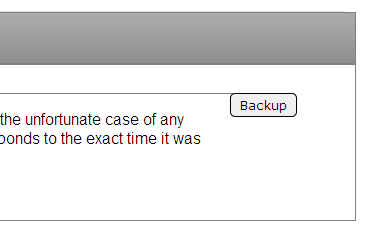
\includegraphics{backupButton.png}
	\end{center}
	\caption{The backup button.}
	\label{backupButton}
\end{figure}
\begin{figure}[h!]
	\begin{center}
	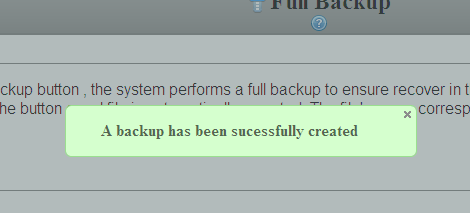
\includegraphics{backupConfirmation.png}
	\end{center}
	\caption{The backup confirmation message.}
	\label{backupConfirmation}
\end{figure}

\subsection{Backing Up Data Manually}
\label{sec:manualBackup}

\par \noindent \hspace*{1cm} Users are also able to create backups manually through MySQL.  This method should only be used by advanced users that are comfortable using the windows command line.  To begin, open a command prompt and navigate to the \verb|bin| directory of your current MySQL installation.  If you do not know where the MySQL installation directory is, please consult the person that installed it. Figure~\ref{binPath} shows an example containing a possible default location.

\begin{figure}[h!]
	\begin{center}
	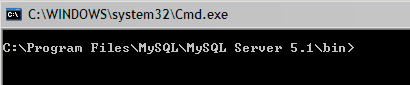
\includegraphics{backupPath.png}
	\end{center}
	\caption{A possible location of the MySQL bin directory.}
	\label{binPath}
\end{figure}

\par \noindent \hspace*{1cm} To create a new backup, enter the following command. Ensure you replace \verb|[outputPath]| with the full path and file location you want for the new backup file, and it should end with the \verb|.sql| extension for easy restoration at a later date. Replace \verb|[errorLogPath]| with the path and file where you would like to keep a log of any errors that may occur during the backup process.
\bigskip
\par \noindent \textbf{mysqldump --databases WebAgenda -u WABroker -ppassword --single-transaction --skip-extended-insert --complete-insert --log-error=[errorLogPath] --result-file=[outputPath]}
\bigskip
\par \noindent \hspace*{1cm} Any errors in either the structure of the command, or in MySQL as it attempts to process the backup will be printed to the command line.  Troubleshooting these errors is outside the scope of this document.  If there are no errors, the command will complete silently and the new backup file will be created

\section{Restoring Backups} 

\par \noindent \hspace*{1cm} Backup restorations can not be done remotely.  Users must be physically at the server to restore backups, ensuring that if there are problems during the restoration they will be able to troubleshoot and fix them. As with manual backups, restorations should only be carried out by users comfortable with the command line, and that are also skilled in the use of MySQL Server and database maintenance.
\bigskip
\par \noindent \hspace*{1cm} Unlike the commands used to create backups, restorations will immediately affect any users that are currently using WebAgenda, and it is \textit{highly} recommended that the WebAgenda system be temporarly brought offline in Glassfish Server until the restoration is complete.
\bigskip
\par \noindent \hspace*{1cm} Any new data that has been created in WebAgenda since the last backup was made will be \textbf{lost} when restoring to a previous state.  As such it is recommended that these backups only be used when absolutely necessary, after normal database recovery procedures have failed to fix a damaged database.
\bigskip
\par \noindent \hspace*{1cm} To restore a backup, navigate to the MySQL \verb|bin| directory as described in Section \ref{sec:manualBackup}.  From here, you may import the backup in one of two ways.

\begin{itemize}
 \item From the Windows command-line. To do this, enter the command "\verb|mysql -u root -p < [backupFile]|", replacing \verb|[backupFile]| with the absolute path to your backup file.
 \item From the MySQL command-line.  First enter MySQL by using the command "\verb|mysql|" without any arguments/options. You will be required to enter a username/password.  Once on the MySQL command-line, issue the command "\verb|source [backupFile]|", replacing \verb|[backupFile]| with the absolute path to your backup file.
\end{itemize}

\par \noindent \hspace*{1cm} For either option, the command must be run with the \verb|root| user, or a user in the MySQL database that has the permissions required on the WebAgenda database to \verb|ADD| or \verb|DROP| tables, and \verb|INSERT| new data.  If successful, the commands will execute silently and without error.  All data should now be rolled back to its state at the time the backup was made.

\chapter{Potential and Known Issues}

\section{Features Not Implemented}

\section{Bugs and System Limitations}

\chapter{Development and Authors}

\par \noindent \hspace*{1cm} WebAgenda \textcopyright  \space was produced in 2009 - 2010 at the Southern Alberta Institute of Technology (SAIT) as part of the Capstone Project for Information Technology. Copyrights of WebAgenda are held by the following authors and developers in association with SAIT and the project is licensed under the GNU Public License Version 2. (See below)

\section{Mark Hazlett}


Interface Developer \newline
Graphic Designer \newline
Project Manager \newline
Mac OS-X Developer

\section{Noorin Hassan}

Quality Assurance \newline
Interface Developer \newline
Documentation Assistant \newline
Windows Developer

\section{Daniel Wehr}

Database Developer \newline
Programming Lead \newline
System Designer \newline
Windows Developer

\section{Daniel Kettle}

Database Designer \newline
Programming Assistant \newline
Documentation Lead \newline
GNU/Linux Developer


\appendix

\chapter{Licenses}

\section{GNU Public License v2}

\par \noindent \hspace*{1cm} MySQL Community Edition and WebAgenda are both licensed under the GPL 2 License as follows:

%\documentclass[11pt]{article}

\title{GNU GENERAL PUBLIC LICENSE}
\date{Version 2, June 1991}

%\begin{document}
%\maketitle

\begin{center}
{\parindent 0in

Copyright \copyright\ 1989, 1991 Free Software Foundation, Inc.

\bigskip

51 Franklin Street, Fifth Floor, Boston, MA  02110-1301, USA

\bigskip

Everyone is permitted to copy and distribute verbatim copies
of this license document, but changing it is not allowed.
}
\end{center}

\begin{center}
{\bf\large Preamble}
\end{center}


The licenses for most software are designed to take away your freedom to
share and change it.  By contrast, the GNU General Public License is
intended to guarantee your freedom to share and change free software---to
make sure the software is free for all its users.  This General Public
License applies to most of the Free Software Foundation's software and to
any other program whose authors commit to using it.  (Some other Free
Software Foundation software is covered by the GNU Library General Public
License instead.)  You can apply it to your programs, too.

When we speak of free software, we are referring to freedom, not price.
Our General Public Licenses are designed to make sure that you have the
freedom to distribute copies of free software (and charge for this service
if you wish), that you receive source code or can get it if you want it,
that you can change the software or use pieces of it in new free programs;
and that you know you can do these things.

To protect your rights, we need to make restrictions that forbid anyone to
deny you these rights or to ask you to surrender the rights.  These
restrictions translate to certain responsibilities for you if you
distribute copies of the software, or if you modify it.

For example, if you distribute copies of such a program, whether gratis or
for a fee, you must give the recipients all the rights that you have.  You
must make sure that they, too, receive or can get the source code.  And
you must show them these terms so they know their rights.

We protect your rights with two steps: (1) copyright the software, and (2)
offer you this license which gives you legal permission to copy,
distribute and/or modify the software.

Also, for each author's protection and ours, we want to make certain that
everyone understands that there is no warranty for this free software.  If
the software is modified by someone else and passed on, we want its
recipients to know that what they have is not the original, so that any
problems introduced by others will not reflect on the original authors'
reputations.

Finally, any free program is threatened constantly by software patents.
We wish to avoid the danger that redistributors of a free program will
individually obtain patent licenses, in effect making the program
proprietary.  To prevent this, we have made it clear that any patent must
be licensed for everyone's free use or not licensed at all.

The precise terms and conditions for copying, distribution and
modification follow.

\begin{center}
{\Large \sc Terms and Conditions For Copying, Distribution and
  Modification}
\end{center}


%\renewcommand{\theenumi}{\alpha{enumi}}
\begin{enumerate}

\addtocounter{enumi}{-1}

\item 

This License applies to any program or other work which contains a notice
placed by the copyright holder saying it may be distributed under the
terms of this General Public License.  The ``Program'', below, refers to
any such program or work, and a ``work based on the Program'' means either
the Program or any derivative work under copyright law: that is to say, a
work containing the Program or a portion of it, either verbatim or with
modifications and/or translated into another language.  (Hereinafter,
translation is included without limitation in the term ``modification''.)
Each licensee is addressed as ``you''.

Activities other than copying, distribution and modification are not
covered by this License; they are outside its scope.  The act of
running the Program is not restricted, and the output from the Program
is covered only if its contents constitute a work based on the
Program (independent of having been made by running the Program).
Whether that is true depends on what the Program does.

\item You may copy and distribute verbatim copies of the Program's source
  code as you receive it, in any medium, provided that you conspicuously
  and appropriately publish on each copy an appropriate copyright notice
  and disclaimer of warranty; keep intact all the notices that refer to
  this License and to the absence of any warranty; and give any other
  recipients of the Program a copy of this License along with the Program.

You may charge a fee for the physical act of transferring a copy, and you
may at your option offer warranty protection in exchange for a fee.

\item

You may modify your copy or copies of the Program or any portion
of it, thus forming a work based on the Program, and copy and
distribute such modifications or work under the terms of Section 1
above, provided that you also meet all of these conditions:

\begin{enumerate}

\item 

You must cause the modified files to carry prominent notices stating that
you changed the files and the date of any change.

\item

You must cause any work that you distribute or publish, that in
whole or in part contains or is derived from the Program or any
part thereof, to be licensed as a whole at no charge to all third
parties under the terms of this License.

\item
If the modified program normally reads commands interactively
when run, you must cause it, when started running for such
interactive use in the most ordinary way, to print or display an
announcement including an appropriate copyright notice and a
notice that there is no warranty (or else, saying that you provide
a warranty) and that users may redistribute the program under
these conditions, and telling the user how to view a copy of this
License.  (Exception: if the Program itself is interactive but
does not normally print such an announcement, your work based on
the Program is not required to print an announcement.)

\end{enumerate}


These requirements apply to the modified work as a whole.  If
identifiable sections of that work are not derived from the Program,
and can be reasonably considered independent and separate works in
themselves, then this License, and its terms, do not apply to those
sections when you distribute them as separate works.  But when you
distribute the same sections as part of a whole which is a work based
on the Program, the distribution of the whole must be on the terms of
this License, whose permissions for other licensees extend to the
entire whole, and thus to each and every part regardless of who wrote it.

Thus, it is not the intent of this section to claim rights or contest
your rights to work written entirely by you; rather, the intent is to
exercise the right to control the distribution of derivative or
collective works based on the Program.

In addition, mere aggregation of another work not based on the Program
with the Program (or with a work based on the Program) on a volume of
a storage or distribution medium does not bring the other work under
the scope of this License.

\item
You may copy and distribute the Program (or a work based on it,
under Section 2) in object code or executable form under the terms of
Sections 1 and 2 above provided that you also do one of the following:

\begin{enumerate}

\item

Accompany it with the complete corresponding machine-readable
source code, which must be distributed under the terms of Sections
1 and 2 above on a medium customarily used for software interchange; or,

\item

Accompany it with a written offer, valid for at least three
years, to give any third party, for a charge no more than your
cost of physically performing source distribution, a complete
machine-readable copy of the corresponding source code, to be
distributed under the terms of Sections 1 and 2 above on a medium
customarily used for software interchange; or,

\item

Accompany it with the information you received as to the offer
to distribute corresponding source code.  (This alternative is
allowed only for noncommercial distribution and only if you
received the program in object code or executable form with such
an offer, in accord with Subsection b above.)

\end{enumerate}


The source code for a work means the preferred form of the work for
making modifications to it.  For an executable work, complete source
code means all the source code for all modules it contains, plus any
associated interface definition files, plus the scripts used to
control compilation and installation of the executable.  However, as a
special exception, the source code distributed need not include
anything that is normally distributed (in either source or binary
form) with the major components (compiler, kernel, and so on) of the
operating system on which the executable runs, unless that component
itself accompanies the executable.

If distribution of executable or object code is made by offering
access to copy from a designated place, then offering equivalent
access to copy the source code from the same place counts as
distribution of the source code, even though third parties are not
compelled to copy the source along with the object code.

\item
You may not copy, modify, sublicense, or distribute the Program
except as expressly provided under this License.  Any attempt
otherwise to copy, modify, sublicense or distribute the Program is
void, and will automatically terminate your rights under this License.
However, parties who have received copies, or rights, from you under
this License will not have their licenses terminated so long as such
parties remain in full compliance.

\item
You are not required to accept this License, since you have not
signed it.  However, nothing else grants you permission to modify or
distribute the Program or its derivative works.  These actions are
prohibited by law if you do not accept this License.  Therefore, by
modifying or distributing the Program (or any work based on the
Program), you indicate your acceptance of this License to do so, and
all its terms and conditions for copying, distributing or modifying
the Program or works based on it.

\item
Each time you redistribute the Program (or any work based on the
Program), the recipient automatically receives a license from the
original licensor to copy, distribute or modify the Program subject to
these terms and conditions.  You may not impose any further
restrictions on the recipients' exercise of the rights granted herein.
You are not responsible for enforcing compliance by third parties to
this License.

\item
If, as a consequence of a court judgment or allegation of patent
infringement or for any other reason (not limited to patent issues),
conditions are imposed on you (whether by court order, agreement or
otherwise) that contradict the conditions of this License, they do not
excuse you from the conditions of this License.  If you cannot
distribute so as to satisfy simultaneously your obligations under this
License and any other pertinent obligations, then as a consequence you
may not distribute the Program at all.  For example, if a patent
license would not permit royalty-free redistribution of the Program by
all those who receive copies directly or indirectly through you, then
the only way you could satisfy both it and this License would be to
refrain entirely from distribution of the Program.

If any portion of this section is held invalid or unenforceable under
any particular circumstance, the balance of the section is intended to
apply and the section as a whole is intended to apply in other
circumstances.

It is not the purpose of this section to induce you to infringe any
patents or other property right claims or to contest validity of any
such claims; this section has the sole purpose of protecting the
integrity of the free software distribution system, which is
implemented by public license practices.  Many people have made
generous contributions to the wide range of software distributed
through that system in reliance on consistent application of that
system; it is up to the author/donor to decide if he or she is willing
to distribute software through any other system and a licensee cannot
impose that choice.

This section is intended to make thoroughly clear what is believed to
be a consequence of the rest of this License.

\item
If the distribution and/or use of the Program is restricted in
certain countries either by patents or by copyrighted interfaces, the
original copyright holder who places the Program under this License
may add an explicit geographical distribution limitation excluding
those countries, so that distribution is permitted only in or among
countries not thus excluded.  In such case, this License incorporates
the limitation as if written in the body of this License.

\item
The Free Software Foundation may publish revised and/or new versions
of the General Public License from time to time.  Such new versions will
be similar in spirit to the present version, but may differ in detail to
address new problems or concerns.

Each version is given a distinguishing version number.  If the Program
specifies a version number of this License which applies to it and ``any
later version'', you have the option of following the terms and conditions
either of that version or of any later version published by the Free
Software Foundation.  If the Program does not specify a version number of
this License, you may choose any version ever published by the Free Software
Foundation.

\item
If you wish to incorporate parts of the Program into other free
programs whose distribution conditions are different, write to the author
to ask for permission.  For software which is copyrighted by the Free
Software Foundation, write to the Free Software Foundation; we sometimes
make exceptions for this.  Our decision will be guided by the two goals
of preserving the free status of all derivatives of our free software and
of promoting the sharing and reuse of software generally.

\begin{center}
{\Large\sc
No Warranty
}
\end{center}

\item
{\sc Because the program is licensed free of charge, there is no warranty
for the program, to the extent permitted by applicable law.  Except when
otherwise stated in writing the copyright holders and/or other parties
provide the program ``as is'' without warranty of any kind, either expressed
or implied, including, but not limited to, the implied warranties of
merchantability and fitness for a particular purpose.  The entire risk as
to the quality and performance of the program is with you.  Should the
program prove defective, you assume the cost of all necessary servicing,
repair or correction.}

\item
{\sc In no event unless required by applicable law or agreed to in writing
will any copyright holder, or any other party who may modify and/or
redistribute the program as permitted above, be liable to you for damages,
including any general, special, incidental or consequential damages arising
out of the use or inability to use the program (including but not limited
to loss of data or data being rendered inaccurate or losses sustained by
you or third parties or a failure of the program to operate with any other
programs), even if such holder or other party has been advised of the
possibility of such damages.}

\end{enumerate}


\begin{center}
{\Large\sc End of Terms and Conditions}
\end{center}


\pagebreak[2]

\section*{Appendix: How to Apply These Terms to Your New Programs}

If you develop a new program, and you want it to be of the greatest
possible use to the public, the best way to achieve this is to make it
free software which everyone can redistribute and change under these
terms.

  To do so, attach the following notices to the program.  It is safest to
  attach them to the start of each source file to most effectively convey
  the exclusion of warranty; and each file should have at least the
  ``copyright'' line and a pointer to where the full notice is found.

\begin{quote}
one line to give the program's name and a brief idea of what it does. \\
Copyright (C) yyyy  name of author \\

This program is free software; you can redistribute it and/or modify
it under the terms of the GNU General Public License as published by
the Free Software Foundation; either version 2 of the License, or
(at your option) any later version.

This program is distributed in the hope that it will be useful,
but WITHOUT ANY WARRANTY; without even the implied warranty of
MERCHANTABILITY or FITNESS FOR A PARTICULAR PURPOSE.  See the
GNU General Public License for more details.

You should have received a copy of the GNU General Public License
along with this program; if not, write to the Free Software
Foundation, Inc., 51 Franklin Street, Fifth Floor, Boston, MA  02110-1301, USA.
\end{quote}

Also add information on how to contact you by electronic and paper mail.

If the program is interactive, make it output a short notice like this
when it starts in an interactive mode:

\begin{quote}
Gnomovision version 69, Copyright (C) yyyy  name of author \\
Gnomovision comes with ABSOLUTELY NO WARRANTY; for details type `show w'. \\
This is free software, and you are welcome to redistribute it
under certain conditions; type `show c' for details.
\end{quote}


The hypothetical commands {\tt show w} and {\tt show c} should show the
appropriate parts of the General Public License.  Of course, the commands
you use may be called something other than {\tt show w} and {\tt show c};
they could even be mouse-clicks or menu items---whatever suits your
program.

You should also get your employer (if you work as a programmer) or your
school, if any, to sign a ``copyright disclaimer'' for the program, if
necessary.  Here is a sample; alter the names:

\begin{quote}
Yoyodyne, Inc., hereby disclaims all copyright interest in the program \\
`Gnomovision' (which makes passes at compilers) written by James Hacker. \\

signature of Ty Coon, 1 April 1989 \\
Ty Coon, President of Vice
\end{quote}


This General Public License does not permit incorporating your program
into proprietary programs.  If your program is a subroutine library, you
may consider it more useful to permit linking proprietary applications
with the library.  If this is what you want to do, use the GNU Library
General Public License instead of this License.

%\end{document}


\newpage

\section{Sun Microsystems License}

\par \noindent \hspace*{1cm} Java EE 6 and Glassfish in addition to other components in the installer are licensed as follows:

\title{GNU GENERAL PUBLIC LICENSE}
\date{Version 2, June 1991}
\begin{verbatim}


\end{verbatim}


\par \noindent Sun Microsystems, Inc. ("Sun") ENTITLEMENT for SOFTWARE
\bigskip 
\par \noindent Licensee/Company: Entity receiving Software.
\bigskip 
\par \noindent Effective Date: Date of delivery of the Software to You.
\bigskip 
\par \noindent Software: Java Platform, Enterprise Edition 6 Web Profile SDK, which includes the following: 
\bigskip
\par \noindent (i)     Sun GlassFish Enterprise Server v3 Web Profile
\par \noindent (ii)    Java EE 6 Samples 
\par \noindent (iv)    First Cup - Your First Cup: An Introduction to the Java EE Platform 
\par \noindent (v)     API Documentation
\bigskip 
\par \noindent License Term:  Perpetual (subject to termination under the SLA)
\bigskip 
\par \noindent Licensed Unit: Software Copy
\bigskip 
\par \noindent Licensed unit Count: Unlimited
\bigskip 
\par \noindent Permitted Uses:
\bigskip 
\par \noindent 1. You may reproduce and use the Software for Your own Individual, Commercial, Service Provider, or Research and Instructional Use for the purposes of designing, developing, testing, and running Your applets and application ("Programs").
\bigskip 
\par \noindent 2. Subject to the terms and conditions of this Agreement and restrictions and exceptions set forth in the Software's documentation, You may reproduce and distribute portions of Software identified as a redistributable in the documentation ("Redistributable"), provided that:
\bigskip 
\par \noindent (a) You distribute Redistributable complete and unmodified and only bundled as part of Your Programs, 
\bigskip 
\par \noindent (b) Your Programs add significant and primary functionality to the Redistributable, 
\bigskip 
\par \noindent (c) You distribute Redistributable for the sole purpose of running Your Programs,
\bigskip 
\par \noindent (d) You do not distribute additional software intended to replace any component(s) of the Redistributable,
\bigskip 
\par \noindent (e) You do not remove or alter any proprietary legends or notices contained in or on the Redistributable.
 \bigskip 
\par \noindent (f) You only distribute the Redistributable subject to a license agreement that protects Sun's interests consistent with the terms contained in this Agreement, and
\bigskip 
\par \noindent (g) You agree to defend and indemnify Sun and its licensors from and against any damages, costs, liabilities, settlement amounts and/or expenses  (including attorneys' fees) incurred in connection with any claim, lawsuit or action by any third party that arises or results from the use or distribution of any and all Programs and/or Redistributable.
\bigskip 
\par \noindent 3. Java Technology Restrictions.  You may not create, modify, or change the behavior of, or authorize your licensees to create, modify, or change the behavior of, classes, interfaces, or subpackages that are in any way identified as "java", "javax", "sun" or similar convention as specified by Sun in any naming convention designation.
\bigskip 
\par \noindent 4. No Diagnostic, Maintenance, Repair or Technical Support Services.  The scope of Your license does not include any right, express or implied, (i) to access, copy, distribute, display or use the Software to provide diagnostic, maintenance, repair or technical support services for Sun software or Sun hardware on behalf of any third party for Your direct or indirect commercial gain or advantage, without Sun's prior written authorization, or (ii) for any third party to access, copy, distribute, display or use the Software to provide diagnostic, maintenance, repair or technical support services for Sun software or Sun hardware on Your behalf for such party's direct or indirect commercial gain or advantage, without Sun's prior written authorization. The limitations set forth in this paragraph apply to any and all error corrections, patches, updates, and upgrades to the Software You may receive, access, download or otherwise obtain from Sun.
\bigskip 
\par \noindent 5) Records and Documentation.  During the term of the SLA and Entitlement, and for a period of three (3) years thereafter, You agree to keep proper records and documentation of Your compliance with the SLA and Entitlement. Upon Sun's reasonable request, You will provide copies of such records and documentation to Sun for the purpose of confirming Your compliance with the terms and conditions of the SLA and Entitlement. This section will survive any termination of the SLA and Entitlement. You may terminate this SLA and Entitlement at any time by destroying all copies of the Software in which case the obligations set forth in Section 7 of the SLA shall apply.
\bigskip 
\bigskip 
\par \noindent Sun Microsystems, Inc. ("Sun")
\par \noindent SOFTWARE LICENSE AGREEMENT
\bigskip 
\par \noindent READ THE TERMS OF THIS AGREEMENT ("AGREEMENT") CAREFULLY BEFORE OPENING SOFTWARE MEDIA PACKAGE. BY OPENING SOFTWARE MEDIA PACKAGE, YOU AGREE TO THE TERMS OF THIS AGREEMENT. IF YOU ARE ACCESSING SOFTWARE ELECTRONICALLY, INDICATE YOUR ACCEPTANCE OF THESE TERMS BY SELECTING THE "ACCEPT" BUTTON AT THE END OF THIS AGREEMENT. IF YOU DO NOT AGREE TO ALL OF THE TERMS, PROMPTLY RETURN THE UNUSED SOFTWARE TO YOUR PLACE OF PURCHASE FOR A REFUND OR, IF SOFTWARE IS ACCESSED ELECTRONICALLY, SELECT THE "DECLINE" (OR "EXIT") BUTTON AT THE END OF THIS AGREEMENT. IF YOU HAVE SEPARATELY AGREED TO LICENSE TERMS ("MASTER TERMS") FOR YOUR LICENSE TO THIS SOFTWARE, THEN SECTIONS 1-6 OF THIS AGREEMENT ("SUPPLEMENTAL LICENSE TERMS") SHALL SUPPLEMENT AND SUPERSEDE THE MASTER TERMS IN RELATION TO THIS SOFTWARE.
\bigskip 
\par \noindent 1.      Definitions.
\bigskip 
\par \noindent (a)     "Entitlement" means the collective set of applicable documents authorized by Sun evidencing your obligation to pay associated fees (if any) for the license, associated Services, and the authorized scope of use of Software under this Agreement.
\bigskip 
\par \noindent (b)     "Licensed Unit" means the unit of measure by which your use of Software and/or Service is licensed, as described in your Entitlement.
\bigskip 
\par \noindent (c)     "Permitted Use" means the licensed Software use(s) authorized in this Agreement as specified in your Entitlement. The Permitted Use for any bundled Sun software not specified in your Entitlement will be evaluation use as provided in Section 3.
\bigskip 
\par \noindent (d)     "Service" means the service(s) that Sun or its delegate will provide, if any, as selected in your Entitlement and as further described in the applicable service listings at www.sun.com/service/servicelist.
\bigskip 
\par \noindent (e)     "Software" means the Sun software described in your Entitlement. Also, certain software may be included for evaluation use under Section 3. 
\bigskip 
\par \noindent (f)     "You" and "Your" means the individual or legal entity specified in the Entitlement, or for evaluation purposes, the entity performing the evaluation.
\bigskip 
\par \noindent 2.      License Grant and Entitlement.
\bigskip 
\par \noindent Subject to the terms of your Entitlement, Sun grants you a nonexclusive, nontransferable limited license to use Software for its Permitted Use for the license term. Your Entitlement will specify (a) Software licensed, (b) the Permitted Use, (c) the license term, and (d) the Licensed Units. 
\bigskip 
\par \noindent Additionally, if your Entitlement includes Services, then it will also specify the (e) Service and (f) service term. 
\bigskip 
\par \noindent If your rights to Software or Services are limited in duration and the date such rights begin is other than the purchase date, your Entitlement will provide that beginning date(s).
\bigskip 
\par \noindent The Entitlement may be delivered to you in various ways depending on the manner in which you obtain Software and Services, for example, the Entitlement may be provided in your receipt, invoice or your contract with Sun or authorized Sun reseller. It may also be in electronic format if you download Software.
\bigskip 
\par \noindent 3.      Permitted Use.
\bigskip 
\par \noindent As selected in your Entitlement, one or more of the following Permitted Uses will apply to your use of Software. Unless you have an Entitlement that expressly permits it, you may not use Software for any of the other Permitted Uses. If you don't have an Entitlement, or if your Entitlement doesn't cover additional software delivered to you, then such software is for your Evaluation Use.
\bigskip 
\par \noindent (a) Evaluation Use. You may evaluate Software internally for a period of 90 days from your first use. 
\bigskip 
\par \noindent (b) Research and Instructional Use. You may use Software internally to design, develop and test, and also to provide instruction on such uses.
\bigskip 
\par \noindent (c) Individual Use. You may use Software internally for personal, individual use.
\bigskip 
\par \noindent (d) Commercial Use. You may use Software internally for your own commercial purposes. 
\bigskip 
\par \noindent (e) Service Provider Use. You may make Software functionality accessible (but not by providing Software itself or through outsourcing services) to your end users in an extranet deployment, but not to your affiliated companies or to government agencies.
\bigskip 
\par \noindent 4.      Licensed Units.
\bigskip 
\par \noindent Your Permitted Use is limited to the number of Licensed Units stated in your Entitlement. If you require additional Licensed Units, you will need additional Entitlement(s).
\bigskip 
\par \noindent 5.      Restrictions.
\bigskip 
\par \noindent (a) The copies of Software provided to you under this Agreement are licensed, not sold, to you by Sun. Sun reserves all rights not expressly granted. (b) You may make a single archival copy of Software, but otherwise may not copy, modify, or distribute Software. However if the Sun documentation accompanying Software lists specific portions of Software, such as header files, class libraries, reference source code, and/or redistributable files, that may be handled differently, you may do so only as provided in the Sun documentation. (c) You may not rent, lease, lend or encumber Software. (d) Unless enforcement is prohibited by applicable law, you may not decompile, or reverse engineer Software. (e) The terms and conditions of this Agreement will apply to any Software updates, provided to you at Sun's discretion, that replace and/or supplement the original Software, unless such update contains a separate license. (f) You may not publish or provide the results of any benchmark or comparison tests run on Software to any third party without the prior written consent of Sun. (g) Software is confidential and copyrighted. (h) Unless otherwise specified, if Software is delivered with embedded or bundled software that enables functionality of Software, you may not use such software on a stand-alone basis or use any portion of such software to interoperate with any program(s) other than Software. (i) Software may contain programs that perform automated collection of system data and/or automated software updating services. System data collected through such programs may be used by Sun, its subcontractors, and its service delivery partners for the purpose of providing you with remote system services and/or improving Sun's software and systems. (j) Software is not designed, licensed or intended for use in the design, construction, operation or maintenance of any nuclear facility and Sun and its licensors disclaim any express or implied warranty of fitness for such uses. (k) No right, title or interest in or to any trademark, service mark, logo or trade name of Sun or its licensors is granted under this Agreement.
\bigskip 
\par \noindent 6.      Java Compatibility and Open Source.
\bigskip 
\par \noindent Software may contain Java technology. You may not create additional classes to, or modifications of, the Java technology, except under compatibility requirements available under a separate agreement available at www.java.net.
\bigskip 
\par \noindent Sun supports and benefits from the global community of open source developers, and thanks the community for its important contributions and open standards-based technology, which Sun has adopted into many of its products.
\bigskip 
\par \noindent Please note that portions of Software may be provided with notices and open source licenses from such communities and third parties that govern the use of those portions, and any licenses granted hereunder do not alter any rights and obligations you may have under such open source licenses, however, the disclaimer of warranty and limitation of liability provisions in this Agreement will apply to all Software in this distribution.
\bigskip 
\par \noindent 7.      Term and Termination. 
\bigskip 
\par \noindent The license and service term are set forth in your Entitlement(s). Your rights under this Agreement will terminate immediately without notice from Sun if you materially breach it or take any action in derogation of Sun's and/or its licensors' rights to Software. Sun may terminate this Agreement should any Software become, or in Sun's reasonable opinion likely to become, the subject of a claim of intellectual property infringement or trade secret misappropriation. Upon termination, you will cease use of, and destroy, Software and confirm compliance in writing to Sun. Sections 1, 5, 6, 7, and 9-15 will survive termination of the Agreement.
\bigskip 
\par \noindent 8.      Limited Warranty. 
\bigskip 
\par \noindent Sun warrants to you that for a period of 90 days from the date of purchase, as evidenced by a copy of the receipt, the media on which Software is furnished (if any) will be free of defects in materials and workmanship under normal use. Except for the foregoing, Software is provided "AS IS". Your exclusive remedy and Sun's entire liability under this limited warranty will be at Sun's option to replace Software media or refund the fee paid for Software. Some states do not allow limitations on certain implied warranties, so the above may not apply to you. This limited warranty gives you specific legal rights. You may have others, which vary from state to state.
\bigskip 
\par \noindent 9.      Disclaimer of Warranty. 
\bigskip 
\par \noindent UNLESS SPECIFIED IN THIS AGREEMENT, ALL EXPRESS OR IMPLIED CONDITIONS, REPRESENTATIONS AND WARRANTIES, INCLUDING ANY IMPLIED WARRANTY OF MERCHANTABILITY, FITNESS FOR A PARTICULAR PURPOSE OR NON-INFRINGEMENT ARE DISCLAIMED, EXCEPT TO THE EXTENT THAT THESE DISCLAIMERS ARE HELD TO BE LEGALLY INVALID. 
\bigskip 
\par \noindent 10.     Limitation of Liability. 
\bigskip 
\par \noindent TO THE EXTENT NOT PROHIBITED BY LAW, IN NO EVENT WILL SUN OR ITS LICENSORS BE LIABLE FOR ANY LOST REVENUE, PROFIT OR DATA, OR FOR SPECIAL, INDIRECT, CONSEQUENTIAL, INCIDENTAL OR PUNITIVE DAMAGES, HOWEVER CAUSED REGARDLESS OF THE THEORY OF LIABILITY, ARISING OUT OF OR RELATED TO THE USE OF OR INABILITY TO USE SOFTWARE, EVEN IF SUN HAS BEEN ADVISED OF THE POSSIBILITY OF SUCH DAMAGES. In no event will Sun's liability to you, whether in contract, tort (including negligence), or otherwise, exceed the amount paid by you for Software under this Agreement. The foregoing limitations will apply even if the above stated warranty fails of its essential purpose. Some states do not allow the exclusion of incidental or consequential damages, so some of the terms above may not be applicable to you. 
\bigskip 
\par \noindent 11.     Export Regulations. 
\bigskip 
\par \noindent All Software, documents, technical data, and any other materials delivered under this Agreement are subject to U.S. export control laws and may be subject to export or import regulations in other countries. You agree to comply strictly with these laws and regulations and acknowledge that you have the responsibility to obtain any licenses to export, re-export, or import as may be required after delivery to you. 
\bigskip 
\par \noindent 12.     U.S. Government Restricted Rights. 
\bigskip 
\par \noindent If Software is being acquired by or on behalf of the U.S. Government or by a U.S. Government prime contractor or subcontractor (at any tier), then the Government's rights in Software and accompanying documentation will be only as set forth in this Agreement; this is in accordance with 48 CFR 227.7201 through 227.7202-4 (for Department of Defense (DOD) acquisitions) and with 48 CFR 2.101 and 12.212 (for non-DOD acquisitions). 
\bigskip 
\par \noindent 13.     Governing Law. 
\bigskip 
\par \noindent Any action related to this Agreement will be governed by California law and controlling U.S. federal law. No choice of law rules of any jurisdiction will apply. 
\bigskip 
\par \noindent 14.     Severability. 
\bigskip 
\par \noindent If any provision of this Agreement is held to be unenforceable, this Agreement will remain in effect with the provision omitted, unless omission would frustrate the intent of the parties, in which case this Agreement will immediately terminate.
\bigskip 
\par \noindent 15.     Integration. 
\bigskip 
\par \noindent This Agreement, including any terms contained in your Entitlement, is the entire agreement between you and Sun relating to its subject matter. It supersedes all prior or contemporaneous oral or written communications, proposals, representations and warranties and prevails over any conflicting or additional terms of any quote, order, acknowledgment, or other communication between the parties relating to its subject matter during the term of this Agreement. No modification of this Agreement will be binding, unless in writing and signed by an authorized representative of each party.
\bigskip 
\par \noindent Please contact Sun Microsystems, Inc. 4150 Network Circle, Santa Clara, California 95054 if you have questions.
\bigskip 


\end{document}         
